% Options for packages loaded elsewhere
\PassOptionsToPackage{unicode}{hyperref}
\PassOptionsToPackage{hyphens}{url}
\PassOptionsToPackage{dvipsnames,svgnames*,x11names*}{xcolor}
%
\documentclass[
]{article}
\usepackage{lmodern}
\usepackage{amsmath}
\usepackage{ifxetex,ifluatex}
\ifnum 0\ifxetex 1\fi\ifluatex 1\fi=0 % if pdftex
  \usepackage[T1]{fontenc}
  \usepackage[utf8]{inputenc}
  \usepackage{textcomp} % provide euro and other symbols
  \usepackage{amssymb}
\else % if luatex or xetex
  \usepackage{unicode-math}
  \defaultfontfeatures{Scale=MatchLowercase}
  \defaultfontfeatures[\rmfamily]{Ligatures=TeX,Scale=1}
\fi
% Use upquote if available, for straight quotes in verbatim environments
\IfFileExists{upquote.sty}{\usepackage{upquote}}{}
\IfFileExists{microtype.sty}{% use microtype if available
  \usepackage[]{microtype}
  \UseMicrotypeSet[protrusion]{basicmath} % disable protrusion for tt fonts
}{}
\makeatletter
\@ifundefined{KOMAClassName}{% if non-KOMA class
  \IfFileExists{parskip.sty}{%
    \usepackage{parskip}
  }{% else
    \setlength{\parindent}{0pt}
    \setlength{\parskip}{6pt plus 2pt minus 1pt}}
}{% if KOMA class
  \KOMAoptions{parskip=half}}
\makeatother
\usepackage{xcolor}
\IfFileExists{xurl.sty}{\usepackage{xurl}}{} % add URL line breaks if available
\IfFileExists{bookmark.sty}{\usepackage{bookmark}}{\usepackage{hyperref}}
\hypersetup{
  pdftitle={Thema08-week1-mRNA},
  pdfauthor={Miguel Botter van Elburg \& Jurrien de Jong},
  colorlinks=true,
  linkcolor=blue,
  filecolor=Maroon,
  citecolor=Blue,
  urlcolor=Blue,
  pdfcreator={LaTeX via pandoc}}
\urlstyle{same} % disable monospaced font for URLs
\usepackage[margin=1in]{geometry}
\usepackage{color}
\usepackage{fancyvrb}
\newcommand{\VerbBar}{|}
\newcommand{\VERB}{\Verb[commandchars=\\\{\}]}
\DefineVerbatimEnvironment{Highlighting}{Verbatim}{commandchars=\\\{\}}
% Add ',fontsize=\small' for more characters per line
\usepackage{framed}
\definecolor{shadecolor}{RGB}{248,248,248}
\newenvironment{Shaded}{\begin{snugshade}}{\end{snugshade}}
\newcommand{\AlertTok}[1]{\textcolor[rgb]{0.94,0.16,0.16}{#1}}
\newcommand{\AnnotationTok}[1]{\textcolor[rgb]{0.56,0.35,0.01}{\textbf{\textit{#1}}}}
\newcommand{\AttributeTok}[1]{\textcolor[rgb]{0.77,0.63,0.00}{#1}}
\newcommand{\BaseNTok}[1]{\textcolor[rgb]{0.00,0.00,0.81}{#1}}
\newcommand{\BuiltInTok}[1]{#1}
\newcommand{\CharTok}[1]{\textcolor[rgb]{0.31,0.60,0.02}{#1}}
\newcommand{\CommentTok}[1]{\textcolor[rgb]{0.56,0.35,0.01}{\textit{#1}}}
\newcommand{\CommentVarTok}[1]{\textcolor[rgb]{0.56,0.35,0.01}{\textbf{\textit{#1}}}}
\newcommand{\ConstantTok}[1]{\textcolor[rgb]{0.00,0.00,0.00}{#1}}
\newcommand{\ControlFlowTok}[1]{\textcolor[rgb]{0.13,0.29,0.53}{\textbf{#1}}}
\newcommand{\DataTypeTok}[1]{\textcolor[rgb]{0.13,0.29,0.53}{#1}}
\newcommand{\DecValTok}[1]{\textcolor[rgb]{0.00,0.00,0.81}{#1}}
\newcommand{\DocumentationTok}[1]{\textcolor[rgb]{0.56,0.35,0.01}{\textbf{\textit{#1}}}}
\newcommand{\ErrorTok}[1]{\textcolor[rgb]{0.64,0.00,0.00}{\textbf{#1}}}
\newcommand{\ExtensionTok}[1]{#1}
\newcommand{\FloatTok}[1]{\textcolor[rgb]{0.00,0.00,0.81}{#1}}
\newcommand{\FunctionTok}[1]{\textcolor[rgb]{0.00,0.00,0.00}{#1}}
\newcommand{\ImportTok}[1]{#1}
\newcommand{\InformationTok}[1]{\textcolor[rgb]{0.56,0.35,0.01}{\textbf{\textit{#1}}}}
\newcommand{\KeywordTok}[1]{\textcolor[rgb]{0.13,0.29,0.53}{\textbf{#1}}}
\newcommand{\NormalTok}[1]{#1}
\newcommand{\OperatorTok}[1]{\textcolor[rgb]{0.81,0.36,0.00}{\textbf{#1}}}
\newcommand{\OtherTok}[1]{\textcolor[rgb]{0.56,0.35,0.01}{#1}}
\newcommand{\PreprocessorTok}[1]{\textcolor[rgb]{0.56,0.35,0.01}{\textit{#1}}}
\newcommand{\RegionMarkerTok}[1]{#1}
\newcommand{\SpecialCharTok}[1]{\textcolor[rgb]{0.00,0.00,0.00}{#1}}
\newcommand{\SpecialStringTok}[1]{\textcolor[rgb]{0.31,0.60,0.02}{#1}}
\newcommand{\StringTok}[1]{\textcolor[rgb]{0.31,0.60,0.02}{#1}}
\newcommand{\VariableTok}[1]{\textcolor[rgb]{0.00,0.00,0.00}{#1}}
\newcommand{\VerbatimStringTok}[1]{\textcolor[rgb]{0.31,0.60,0.02}{#1}}
\newcommand{\WarningTok}[1]{\textcolor[rgb]{0.56,0.35,0.01}{\textbf{\textit{#1}}}}
\usepackage{graphicx}
\makeatletter
\def\maxwidth{\ifdim\Gin@nat@width>\linewidth\linewidth\else\Gin@nat@width\fi}
\def\maxheight{\ifdim\Gin@nat@height>\textheight\textheight\else\Gin@nat@height\fi}
\makeatother
% Scale images if necessary, so that they will not overflow the page
% margins by default, and it is still possible to overwrite the defaults
% using explicit options in \includegraphics[width, height, ...]{}
\setkeys{Gin}{width=\maxwidth,height=\maxheight,keepaspectratio}
% Set default figure placement to htbp
\makeatletter
\def\fps@figure{htbp}
\makeatother
\setlength{\emergencystretch}{3em} % prevent overfull lines
\providecommand{\tightlist}{%
  \setlength{\itemsep}{0pt}\setlength{\parskip}{0pt}}
\setcounter{secnumdepth}{5}
\usepackage{longtable}
\usepackage{hyperref}
\ifluatex
  \usepackage{selnolig}  % disable illegal ligatures
\fi

\title{Thema08-week1-mRNA}
\author{Miguel Botter van Elburg \& Jurrien de Jong}
\date{2021-05-21}

\begin{document}
\maketitle

\begin{Shaded}
\begin{Highlighting}[]
\NormalTok{data }\OtherTok{\textless{}{-}} \FunctionTok{read.csv}\NormalTok{(}\StringTok{"MPL.csv"}\NormalTok{, }\AttributeTok{na.strings =} \StringTok{"NA"}\NormalTok{)}

\NormalTok{medians }\OtherTok{\textless{}{-}} \FunctionTok{aggregate}\NormalTok{(data[,}\FunctionTok{c}\NormalTok{(}\StringTok{"MPL\_conc"}\NormalTok{,}\StringTok{"mRNA"}\NormalTok{,}\StringTok{"Free\_receptor"}\NormalTok{)],}\FunctionTok{list}\NormalTok{(data}\SpecialCharTok{$}\NormalTok{dose,data}\SpecialCharTok{$}\NormalTok{time), median, }\AttributeTok{na.rm=}\NormalTok{T)}
\FunctionTok{names}\NormalTok{(medians)[}\DecValTok{1}\SpecialCharTok{:}\DecValTok{2}\NormalTok{] }\OtherTok{\textless{}{-}} \FunctionTok{c}\NormalTok{(}\StringTok{"dose"}\NormalTok{,}\StringTok{"time"}\NormalTok{)}
\NormalTok{medians\_01 }\OtherTok{\textless{}{-}} \FunctionTok{subset}\NormalTok{(medians, dose }\SpecialCharTok{==} \FloatTok{0.1} \SpecialCharTok{|}\NormalTok{ dose }\SpecialCharTok{==} \DecValTok{0}\NormalTok{)}
\NormalTok{medians\_03 }\OtherTok{\textless{}{-}} \FunctionTok{subset}\NormalTok{(medians, dose }\SpecialCharTok{==} \FloatTok{0.3} \SpecialCharTok{|}\NormalTok{ dose }\SpecialCharTok{==} \DecValTok{0}\NormalTok{)}
\end{Highlighting}
\end{Shaded}

\hypertarget{introduction}{%
\section{Introduction}\label{introduction}}

Zal een model altijd kloppen? Wanneer we de model data vergelijken met
echte uitgevoerde onderzoeken met ratten kan er duidelijk gezegd worden
of het model daadwerkelijk geldig is. Modellen zijn vooral handig om te
kijken wat er precies gebeurd bij bepaalde scenario's, zo hoeven we ze
niet in het echt uit te voeren, slechts met een simulatie. Het bewijzen
van de geldigheid van het model en het visualiseren van verschillende
scenario's komen in dit onderzoek aan bod.

\hypertarget{goal}{%
\subsection{Goal}\label{goal}}

Het doel is nu voornamelijk om te bekijken wat er gebeurt met de
grafieken als parameters verandert worden ( oftewel er moeten
verschillende scenario's gerunt worden ). Ook zal de geldigheid van het
model op de proef gesteld worden.

\hypertarget{theory}{%
\subsection{Theory}\label{theory}}

Bij een corticosteroïden behandeling wordt een medicijn (hormoon
corticosteroïd) in een gewricht, peesschede of rond de zenuw gebracht.
De corticosteroïden hebben een ontstekingsremmende werking en geven de
geprikkelde zenuwen rust {[}@A{]}.

Enkele voorbeelden van corticosteroïden zijn; Predniso(lo)n,
Dexamethason, (Hydro)cortison, Triamcinolon, Betametason, Fluticason
{[}@B{]}.

De werking van corticosteroïden verschilt. Dit geldt voor sterkte,
toedieningsvorm en mate van bijwerkingen. Het kan voorgeschreven worden
als stootkuur (korte periode een hoge dosering), maar ook langdurig als
onderhoudsbehandeling. In het geval van longpatiënten worden
corticosteroïden gebruikt als ontstekingsremmer en worden ze ingezet bij
allergische reacties op uitwendige prikkels (vb: hooikoorts, eczeem)
{[}@C{]}.

\hypertarget{methods}{%
\section{Methods}\label{methods}}

Over het algemeen biedt de mediaan een beter idee van de data verdeling,
bij steekproefproefgemiddelden mits zij een normaal verdeling volgen.
Aangezien de mediaan robuuster is dan een gemiddelde (mean), want het is
minder afhankelijk van uitbijters/uitschieters, omdat het het middelste
punt is van een gesorteerde reeks cijfers/getallen/gegevens en de scores
niet worden gedeeld door het aantal n.~Een goede illustratie zegt meer
dan duizend woorden, om die reden is het beter om een grafiek van de
mediaan erbij te plotten.

\hypertarget{the-software-model}{%
\subsection{The software model}\label{the-software-model}}

De glucocorticoiden zullen met name meerdere ontstekings geactiveerde
genen uitzetten, die coderen voor cytokines, chemokines, hechtings
moleculen van ontstoken enzymen en receptors (zie Fig 1). Deze genen
zijn aangezet in de luchtwegen door pro-ontstekings transcriptie
factoren, zoals nuclear factor-κB (NF-κB) en activator protein-1 (AP-1),
die normaal gesproken beide worden geactiveerd in de buurt van asthma en
COPD ontstekingen (zie Fig 2).

\begin{Shaded}
\begin{Highlighting}[]
\NormalTok{knitr}\SpecialCharTok{::}\FunctionTok{include\_graphics}\NormalTok{(}\StringTok{\textquotesingle{}Fig1\_week2.jpg\textquotesingle{}}\NormalTok{)}
\end{Highlighting}
\end{Shaded}

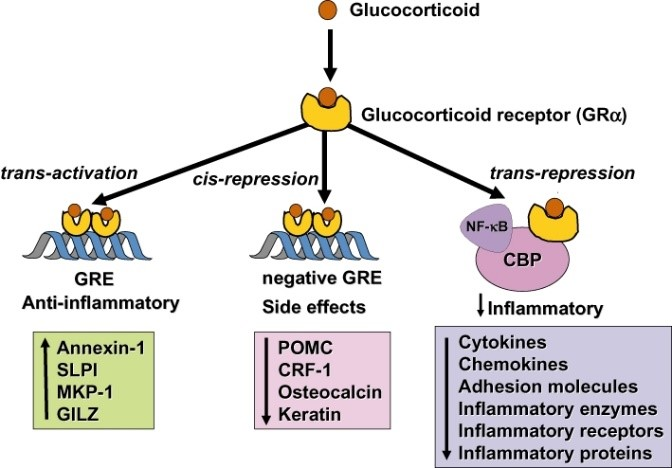
\includegraphics[width=9.33in]{Fig1_week2}

\begin{Shaded}
\begin{Highlighting}[]
\NormalTok{knitr}\SpecialCharTok{::}\FunctionTok{include\_graphics}\NormalTok{(}\StringTok{\textquotesingle{}Fig2\_week2.jpg\textquotesingle{}}\NormalTok{)}
\end{Highlighting}
\end{Shaded}

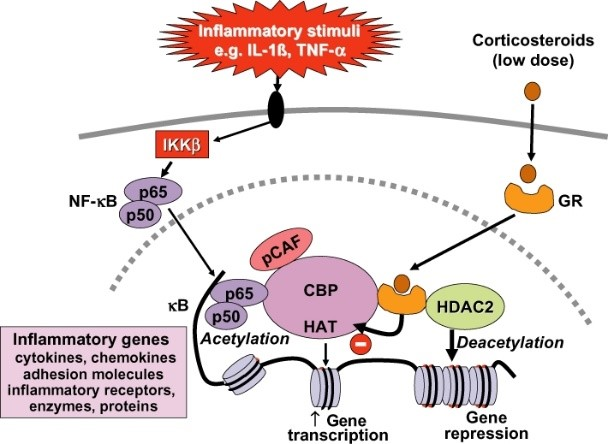
\includegraphics[width=8.44in]{Fig2_week2}

\hypertarget{model-configuration}{%
\subsection{Model configuration}\label{model-configuration}}

De configuratie ( parameters etc ) is te zien in onderstaand
figuur/tabel. Let op. Bij verschillende opgaven worden andere parameters
gebruikt, zoals dat D = 39 bij de onderstaande code block in de
`results' sectie.

\begin{Shaded}
\begin{Highlighting}[]
\NormalTok{knitr}\SpecialCharTok{::}\FunctionTok{include\_graphics}\NormalTok{(}\StringTok{\textquotesingle{}Fig3\_week2.png\textquotesingle{}}\NormalTok{)}
\end{Highlighting}
\end{Shaded}

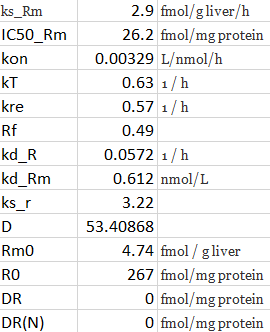
\includegraphics[width=3.75in]{Fig3_week2}

\hypertarget{results}{%
\section{Results}\label{results}}

De vragen die opkomen tijdens het onderzoeken van een biologisch systeem
zal je kunnen beantwoorden aan de hand van een gecreerd model. Hieronder
is de code te zien dat zo'n soort model kan produceren:

\begin{Shaded}
\begin{Highlighting}[]
\CommentTok{\# this function calculates the derivatives and returns it as a list.}
\NormalTok{Glucocorticoid\_func }\OtherTok{\textless{}{-}} \ControlFlowTok{function}\NormalTok{(t, y, parms) \{}
    \FunctionTok{with}\NormalTok{(}\FunctionTok{as.list}\NormalTok{(}\FunctionTok{c}\NormalTok{(y, parms)),\{}
      
      \CommentTok{\# Dit model bevat 4 afgeleide functies:}
      \CommentTok{\# Afgeleide 1:}
  
\NormalTok{      dmRNAr\_dt }\OtherTok{\textless{}{-}}\NormalTok{ ks\_Rm }\SpecialCharTok{*}\NormalTok{ ( }\DecValTok{1} \SpecialCharTok{{-}}\NormalTok{ (DRN }\SpecialCharTok{/}\NormalTok{ (IC50\_Rm }\SpecialCharTok{+}\NormalTok{ DRN))) }\SpecialCharTok{{-}}\NormalTok{ kd\_Rm }\SpecialCharTok{*}\NormalTok{ mRNAr}
  
      \CommentTok{\# Afgeleide 2:}
  
\NormalTok{      dR\_dt }\OtherTok{\textless{}{-}}\NormalTok{ ks\_r }\SpecialCharTok{*}\NormalTok{ mRNAr }\SpecialCharTok{+}\NormalTok{ Rf }\SpecialCharTok{*}\NormalTok{ kre }\SpecialCharTok{*}\NormalTok{ DRN }\SpecialCharTok{{-}}\NormalTok{ kon }\SpecialCharTok{*}\NormalTok{ D }\SpecialCharTok{*}\NormalTok{ R }\SpecialCharTok{{-}}\NormalTok{ kd\_R }\SpecialCharTok{*}\NormalTok{ R}
      
      \CommentTok{\# Afgeleide 3:}
  
\NormalTok{      dDR\_dt }\OtherTok{\textless{}{-}}\NormalTok{ kon }\SpecialCharTok{*}\NormalTok{ D }\SpecialCharTok{*}\NormalTok{ R }\SpecialCharTok{{-}}\NormalTok{ kT }\SpecialCharTok{*}\NormalTok{ DR}
  
      \CommentTok{\# Afgeleide 4:}
  
\NormalTok{      dDRN\_dt }\OtherTok{\textless{}{-}}\NormalTok{ kT }\SpecialCharTok{*}\NormalTok{ DR }\SpecialCharTok{{-}}\NormalTok{ kre }\SpecialCharTok{*}\NormalTok{ DRN}
      
      \FunctionTok{return}\NormalTok{(}\FunctionTok{list}\NormalTok{(}\FunctionTok{c}\NormalTok{(dmRNAr\_dt, dR\_dt, dDR\_dt, dDRN\_dt)))}
\NormalTok{       \}}
\NormalTok{       )}
\NormalTok{\}}
\end{Highlighting}
\end{Shaded}

Question 1.2

\begin{Shaded}
\begin{Highlighting}[]
\FunctionTok{par}\NormalTok{(}\AttributeTok{mfrow =} \FunctionTok{c}\NormalTok{(}\DecValTok{2}\NormalTok{,}\DecValTok{2}\NormalTok{) )}

\CommentTok{\# Set initial values}
\NormalTok{state }\OtherTok{\textless{}{-}} \FunctionTok{c}\NormalTok{(}\AttributeTok{mRNAr =} \FloatTok{4.74}\NormalTok{, }\AttributeTok{R =} \DecValTok{267}\NormalTok{, }\AttributeTok{DR =} \DecValTok{0}\NormalTok{, }\AttributeTok{DRN =} \DecValTok{0}\NormalTok{)}
\NormalTok{t }\OtherTok{\textless{}{-}} \FunctionTok{seq}\NormalTok{(}\DecValTok{0}\NormalTok{, }\DecValTok{168}\NormalTok{, }\AttributeTok{by =} \DecValTok{1}\NormalTok{)}

\CommentTok{\# {-}{-}{-}{-}{-}{-}{-}{-}{-}{-}{-}{-}{-}{-}{-}{-}{-}{-}{-}{-}{-}{-}{-}{-}{-}{-}{-}{-}{-}{-}{-}{-}{-}{-}{-}{-}{-}{-}{-}{-}{-}{-}{-}{-}{-}{-}{-}}
\CommentTok{\# Dose 0.1}

\NormalTok{parameters\_01 }\OtherTok{\textless{}{-}} \FunctionTok{c}\NormalTok{(}\AttributeTok{ks\_Rm =} \FloatTok{2.90}\NormalTok{, }\AttributeTok{IC50\_Rm =} \FloatTok{26.2}\NormalTok{, }\AttributeTok{kon =} \FloatTok{0.00329}\NormalTok{,}
                \AttributeTok{kT =} \FloatTok{0.63}\NormalTok{, }\AttributeTok{kre =} \FloatTok{0.57}\NormalTok{, }\AttributeTok{Rf =} \FloatTok{0.49}\NormalTok{, }\AttributeTok{kd\_R =} \FloatTok{0.0572}\NormalTok{,}
                \AttributeTok{kd\_Rm =} \FloatTok{0.612}\NormalTok{, }\AttributeTok{ks\_r =} \FloatTok{3.22}\NormalTok{, }\AttributeTok{D =} \FloatTok{39.0}\NormalTok{, }\AttributeTok{Rm0 =} \FloatTok{4.74}\NormalTok{,}
                \AttributeTok{DR =} \DecValTok{0}\NormalTok{, }\AttributeTok{DRN =} \DecValTok{0}\NormalTok{)}

\NormalTok{out\_01 }\OtherTok{\textless{}{-}}\NormalTok{ deSolve}\SpecialCharTok{::}\FunctionTok{ode}\NormalTok{(}\AttributeTok{times =}\NormalTok{ t, }\AttributeTok{y =}\NormalTok{ state, }\AttributeTok{parms =}\NormalTok{ parameters\_01,}
                    \AttributeTok{func =}\NormalTok{ Glucocorticoid\_func, }\AttributeTok{method =} \StringTok{"lsoda"}\NormalTok{)}

\NormalTok{out\_01 }\OtherTok{\textless{}{-}} \FunctionTok{as.data.frame}\NormalTok{(out\_01)}

\FunctionTok{plot}\NormalTok{(out\_01}\SpecialCharTok{$}\NormalTok{time, out\_01}\SpecialCharTok{$}\NormalTok{mRNAr,}
     \AttributeTok{main=}\StringTok{"Receptor mRNA by dose 0.1"}\NormalTok{,}
     \AttributeTok{ylab=}\FunctionTok{c}\NormalTok{(}\StringTok{"nmol/L"}\NormalTok{), }\AttributeTok{xlab=}\FunctionTok{c}\NormalTok{(}\StringTok{" Time in hours"}\NormalTok{),}
     \AttributeTok{type=}\StringTok{\textquotesingle{}l\textquotesingle{}}\NormalTok{, }\AttributeTok{lwd =} \DecValTok{2}\NormalTok{, }\AttributeTok{xlim=} \FunctionTok{c}\NormalTok{(}\DecValTok{0}\NormalTok{,}\DecValTok{60}\NormalTok{), }\AttributeTok{ylim=} \FunctionTok{c}\NormalTok{(}\DecValTok{0}\NormalTok{,}\DecValTok{5}\NormalTok{))}

\FunctionTok{lines}\NormalTok{(data}\SpecialCharTok{$}\NormalTok{time, data}\SpecialCharTok{$}\NormalTok{mRNA, }\AttributeTok{type =} \StringTok{"p"}\NormalTok{)}
\FunctionTok{lines}\NormalTok{(medians\_01}\SpecialCharTok{$}\NormalTok{time, medians\_01}\SpecialCharTok{$}\NormalTok{mRNA, }\AttributeTok{type =} \StringTok{"l"}\NormalTok{, }\AttributeTok{col=} \StringTok{"red"}\NormalTok{)}

\FunctionTok{plot}\NormalTok{(out\_01}\SpecialCharTok{$}\NormalTok{time, out\_01}\SpecialCharTok{$}\NormalTok{R,}
     \AttributeTok{main=}\StringTok{"Free receptor mRNA by dose 0.1"}\NormalTok{,}
     \AttributeTok{ylab=}\FunctionTok{c}\NormalTok{(}\StringTok{"nmol/L"}\NormalTok{), }\AttributeTok{xlab=}\FunctionTok{c}\NormalTok{(}\StringTok{" Time in hours"}\NormalTok{),}
     \AttributeTok{type=}\StringTok{\textquotesingle{}l\textquotesingle{}}\NormalTok{, }\AttributeTok{lwd =} \DecValTok{2}\NormalTok{, }\AttributeTok{xlim=} \FunctionTok{c}\NormalTok{(}\DecValTok{0}\NormalTok{,}\DecValTok{60}\NormalTok{), }\AttributeTok{ylim=} \FunctionTok{c}\NormalTok{(}\DecValTok{0}\NormalTok{,}\DecValTok{500}\NormalTok{))}

\FunctionTok{lines}\NormalTok{(data}\SpecialCharTok{$}\NormalTok{time, data}\SpecialCharTok{$}\NormalTok{Free\_receptor, }\AttributeTok{type =} \StringTok{"p"}\NormalTok{)}
\FunctionTok{lines}\NormalTok{(medians\_01}\SpecialCharTok{$}\NormalTok{time, medians\_01}\SpecialCharTok{$}\NormalTok{Free\_receptor, }\AttributeTok{type =} \StringTok{"l"}\NormalTok{, }\AttributeTok{col=} \StringTok{"red"}\NormalTok{)}

\CommentTok{\# {-}{-}{-}{-}{-}{-}{-}{-}{-}{-}{-}{-}{-}{-}{-}{-}{-}{-}{-}{-}{-}{-}{-}{-}{-}{-}{-}{-}{-}{-}{-}{-}{-}{-}{-}}
\CommentTok{\# Dose 0.3}

\NormalTok{parameters\_03 }\OtherTok{\textless{}{-}} \FunctionTok{c}\NormalTok{(}\AttributeTok{ks\_Rm =} \FloatTok{2.90}\NormalTok{, }\AttributeTok{IC50\_Rm =} \FloatTok{26.2}\NormalTok{, }\AttributeTok{kon =} \FloatTok{0.00329}\NormalTok{,}
                \AttributeTok{kT =} \FloatTok{0.63}\NormalTok{, }\AttributeTok{kre =} \FloatTok{0.57}\NormalTok{, }\AttributeTok{Rf =} \FloatTok{0.49}\NormalTok{, }\AttributeTok{kd\_R =} \FloatTok{0.0572}\NormalTok{,}
                \AttributeTok{kd\_Rm =} \FloatTok{0.612}\NormalTok{, }\AttributeTok{ks\_r =} \FloatTok{3.22}\NormalTok{, }\AttributeTok{D =} \DecValTok{107}\NormalTok{, }\AttributeTok{Rm0 =} \FloatTok{4.74}\NormalTok{,}
                \AttributeTok{DR =} \DecValTok{0}\NormalTok{, }\AttributeTok{DRN =} \DecValTok{0}\NormalTok{)}

\NormalTok{out\_03 }\OtherTok{\textless{}{-}}\NormalTok{ deSolve}\SpecialCharTok{::}\FunctionTok{ode}\NormalTok{(}\AttributeTok{times =}\NormalTok{ t, }\AttributeTok{y =}\NormalTok{ state, }\AttributeTok{parms =}\NormalTok{ parameters\_03,}
                    \AttributeTok{func =}\NormalTok{ Glucocorticoid\_func, }\AttributeTok{method =} \StringTok{"lsoda"}\NormalTok{)}

\NormalTok{out\_03 }\OtherTok{\textless{}{-}} \FunctionTok{as.data.frame}\NormalTok{(out\_03)}

\FunctionTok{plot}\NormalTok{(out\_03}\SpecialCharTok{$}\NormalTok{time, out\_03}\SpecialCharTok{$}\NormalTok{mRNAr,}
     \AttributeTok{main=}\StringTok{"Receptor mRNA by dose 0.3"}\NormalTok{,}
     \AttributeTok{ylab=}\FunctionTok{c}\NormalTok{(}\StringTok{"nmol/L"}\NormalTok{), }\AttributeTok{xlab=}\FunctionTok{c}\NormalTok{(}\StringTok{" Time in hours"}\NormalTok{),}
     \AttributeTok{type=}\StringTok{\textquotesingle{}l\textquotesingle{}}\NormalTok{, }\AttributeTok{lwd =} \DecValTok{2}\NormalTok{, }\AttributeTok{xlim=} \FunctionTok{c}\NormalTok{(}\DecValTok{0}\NormalTok{,}\DecValTok{60}\NormalTok{), }\AttributeTok{ylim=} \FunctionTok{c}\NormalTok{(}\DecValTok{0}\NormalTok{,}\DecValTok{5}\NormalTok{))}

\FunctionTok{lines}\NormalTok{(data}\SpecialCharTok{$}\NormalTok{time, data}\SpecialCharTok{$}\NormalTok{mRNA, }\AttributeTok{type =} \StringTok{"p"}\NormalTok{)}
\FunctionTok{lines}\NormalTok{(medians\_01}\SpecialCharTok{$}\NormalTok{time, medians\_01}\SpecialCharTok{$}\NormalTok{mRNA, }\AttributeTok{type =} \StringTok{"l"}\NormalTok{, }\AttributeTok{col=} \StringTok{"red"}\NormalTok{)}

\FunctionTok{plot}\NormalTok{(out\_03}\SpecialCharTok{$}\NormalTok{time, out\_03}\SpecialCharTok{$}\NormalTok{R,}
     \AttributeTok{main=}\StringTok{"Free receptor mRNA by dose 0.3"}\NormalTok{,}
     \AttributeTok{ylab=}\FunctionTok{c}\NormalTok{(}\StringTok{"nmol/L"}\NormalTok{), }\AttributeTok{xlab=}\FunctionTok{c}\NormalTok{(}\StringTok{" Time in hours"}\NormalTok{),}
     \AttributeTok{type=}\StringTok{\textquotesingle{}l\textquotesingle{}}\NormalTok{, }\AttributeTok{lwd =} \DecValTok{2}\NormalTok{, }\AttributeTok{xlim=} \FunctionTok{c}\NormalTok{(}\DecValTok{0}\NormalTok{,}\DecValTok{60}\NormalTok{), }\AttributeTok{ylim=} \FunctionTok{c}\NormalTok{(}\DecValTok{0}\NormalTok{,}\DecValTok{500}\NormalTok{))}

\FunctionTok{lines}\NormalTok{(data}\SpecialCharTok{$}\NormalTok{time, data}\SpecialCharTok{$}\NormalTok{Free\_receptor, }\AttributeTok{type =} \StringTok{"p"}\NormalTok{)}
\FunctionTok{lines}\NormalTok{(medians\_01}\SpecialCharTok{$}\NormalTok{time, medians\_01}\SpecialCharTok{$}\NormalTok{Free\_receptor, }\AttributeTok{type =} \StringTok{"l"}\NormalTok{, }\AttributeTok{col=} \StringTok{"red"}\NormalTok{)}
\end{Highlighting}
\end{Shaded}

\includegraphics{Project-Thema08-week3-Groep2_v1_files/figure-latex/unnamed-chunk-2-1.pdf}

Question 1.3

De resultaten van het model (zwart) komen wel overeen met elkaar,
aangezien de gefitte lijnen (rode experiment data) een gevolg zijn van
de data observaties (zwarte model data). Het onderlinge verschil tussen
de twee model zwarte model-lijnen is mogelijk te verklaren door het
onderlinge verschil in condities van model groepen (sample groups).
Omdat een hogere drug concentratie leidt tot verhoogde kans van
bindingen met mRNA receptoren zal de concentratie mRNA bezette
receptoren bij een hogere dosis (0.3 ipv 0.1) sneller afnemen in een
bepaalde tijd (zie fig Receptor mRNA by dose 0.3) dan bij een lagere
dosis (zie fig Receptor mRNA by dose 0.1) Dat verschil is af te leiden
tussen de grafieken!

Q2.1

De tijdsverloop van het geactiveerde drug-receptor complex is
afhankelijk van de auto-regulatie van de glucorticoide receptor. Hierom
moet de formule die de auto-regulatie van de glucorticoide receptor
variabele bevat worden aangepast, dat is de formule `Afgeleide 1' in de
code chunk `formule\_modellen'. Zie de onderstaande aangepaste functie
van het model en de output daarvan.

(x+1)(x-1) = 0 Bovenstaande vergelijking is alleen waar als x = -1 of x
= 1, omdat dan een van beide producten dan nul is en iets keer nul is
nul.

dmRNAr\_dt \textless- ks\_Rm * ( 1 - (DRN / (IC50\_Rm + DRN))) - kd\_Rm
* mRNAr Wanneer er geen auto-regulatie is van de glucocorticoide
receptor is, betekent het dat de uitkomst nul wordt. Dus de `Afgeleide
1' herleiden we op nul, net als het voorbeeld van (x+1) (x-1)\ldots{}

De parameter ks\_Rm is afhankelijk van ( 1 - (DRN / (IC50\_Rm + DRN) en
wordt nul als ( 1 - (DRN / (IC50\_Rm + DRN) nul is.

Dus moet de volgende vergelijking worden opgelost\ldots{} ks\_Rm * ( 1 -
(DRN / (IC50\_Rm + DRN))) = 0 dus\ldots{} 1 -1*(DRN / (IC50\_Rm + DRN))
= 0 dus\ldots{} 1 = +1(DRN / (IC5\_Rm + DRN)) dus\ldots{} 1 = (DRN /
(IC5\_Rm + DRN))

dus\ldots{} 1 = (0 / (0 + 0)) want 0 / 0 is 1! oplossing: dus de
parameters DRN, IC5\_Rm, DRN zijn nul en de vergelijking kan dus
verwijderd worden.

\begin{Shaded}
\begin{Highlighting}[]
\NormalTok{Glucocorticoid\_func\_2}\FloatTok{.1} \OtherTok{\textless{}{-}} \ControlFlowTok{function}\NormalTok{(t, y, parms) \{}
    \FunctionTok{with}\NormalTok{(}\FunctionTok{as.list}\NormalTok{(}\FunctionTok{c}\NormalTok{(y, parms)),\{}
      
      \CommentTok{\# Dit model bevat 4 afgeleide functies:}
      \CommentTok{\# Afgeleide 1:}
      
\NormalTok{      dmRNAr\_dt }\OtherTok{\textless{}{-}}\NormalTok{ ks\_Rm }\SpecialCharTok{{-}}\NormalTok{ kd\_Rm }\SpecialCharTok{*}\NormalTok{ mRNAr }\CommentTok{\# * (DRN / (IC5\_Rm + DRN)) This has been removed to answer}
                                         \CommentTok{\# the research question}
  
      \CommentTok{\# Afgeleide 2:}
  
\NormalTok{      dR\_dt }\OtherTok{\textless{}{-}}\NormalTok{ ks\_r }\SpecialCharTok{*}\NormalTok{ mRNAr }\SpecialCharTok{+}\NormalTok{ Rf }\SpecialCharTok{*}\NormalTok{ kre }\SpecialCharTok{*}\NormalTok{ DRN }\SpecialCharTok{{-}}\NormalTok{ kon }\SpecialCharTok{*}\NormalTok{ D }\SpecialCharTok{*}\NormalTok{ R }\SpecialCharTok{{-}}\NormalTok{ kd\_R }\SpecialCharTok{*}\NormalTok{ R}
      
      \CommentTok{\# Afgeleide 3:}
  
\NormalTok{      dDR\_dt }\OtherTok{\textless{}{-}}\NormalTok{ kon }\SpecialCharTok{*}\NormalTok{ D }\SpecialCharTok{*}\NormalTok{ R }\SpecialCharTok{{-}}\NormalTok{ kT }\SpecialCharTok{*}\NormalTok{ DR}
  
      \CommentTok{\# Afgeleide 4:}
  
\NormalTok{      dDRN\_dt }\OtherTok{\textless{}{-}}\NormalTok{ kT }\SpecialCharTok{*}\NormalTok{ DR }\SpecialCharTok{{-}}\NormalTok{ kre }\SpecialCharTok{*}\NormalTok{ DRN}
      
      \FunctionTok{return}\NormalTok{(}\FunctionTok{list}\NormalTok{(}\FunctionTok{c}\NormalTok{(dmRNAr\_dt, dR\_dt, dDR\_dt, dDRN\_dt)))}
\NormalTok{       \}}
\NormalTok{       )}
\NormalTok{\}}

\NormalTok{parameters }\OtherTok{\textless{}{-}} \FunctionTok{c}\NormalTok{(}\AttributeTok{ks\_Rm =} \FloatTok{2.90}\NormalTok{, }\AttributeTok{IC50\_Rm =} \FloatTok{26.2}\NormalTok{, }\AttributeTok{kon =} \FloatTok{0.00329}\NormalTok{,}
                \AttributeTok{kT =} \FloatTok{0.63}\NormalTok{, }\AttributeTok{kre =} \FloatTok{0.57}\NormalTok{, }\AttributeTok{Rf =} \FloatTok{0.49}\NormalTok{, }\AttributeTok{kd\_R =} \FloatTok{0.0572}\NormalTok{,}
                \AttributeTok{kd\_Rm =} \FloatTok{0.612}\NormalTok{, }\AttributeTok{ks\_r =} \FloatTok{3.22}\NormalTok{, }\AttributeTok{D =} \DecValTok{53}\NormalTok{, }\AttributeTok{Rm0 =} \FloatTok{4.74}\NormalTok{,}
                \AttributeTok{DR =} \DecValTok{0}\NormalTok{, }\AttributeTok{DRN =} \DecValTok{0}\NormalTok{)}

\NormalTok{t }\OtherTok{=} \FunctionTok{seq}\NormalTok{(}\DecValTok{0}\NormalTok{, }\DecValTok{48}\NormalTok{, }\AttributeTok{by =} \FloatTok{0.1}\NormalTok{)}

\NormalTok{out }\OtherTok{\textless{}{-}}\NormalTok{ deSolve}\SpecialCharTok{::}\FunctionTok{ode}\NormalTok{(}\AttributeTok{times =}\NormalTok{ t, }\AttributeTok{y =}\NormalTok{ state, }\AttributeTok{parms =}\NormalTok{ parameters,}
                    \AttributeTok{func =}\NormalTok{ Glucocorticoid\_func\_2}\FloatTok{.1}\NormalTok{, }\AttributeTok{method =} \StringTok{"lsoda"}\NormalTok{)}


\NormalTok{out }\OtherTok{\textless{}{-}} \FunctionTok{as.data.frame}\NormalTok{(out)}

\FunctionTok{par}\NormalTok{(}\AttributeTok{mfrow=}\FunctionTok{c}\NormalTok{(}\DecValTok{2}\NormalTok{,}\DecValTok{2}\NormalTok{))}
  \FunctionTok{plot}\NormalTok{(out}\SpecialCharTok{$}\NormalTok{time,out}\SpecialCharTok{$}\NormalTok{mRNAr,}\AttributeTok{ylim =} \FunctionTok{c}\NormalTok{(}\DecValTok{0}\NormalTok{,}\DecValTok{5}\NormalTok{), }\AttributeTok{xlab=}\StringTok{"Time"}\NormalTok{,}\AttributeTok{ylab=}\StringTok{"receptor mRNA"}\NormalTok{,}\AttributeTok{type=}\StringTok{"l"}\NormalTok{,}\AttributeTok{lwd=}\DecValTok{2}\NormalTok{)}
  \FunctionTok{plot}\NormalTok{(out}\SpecialCharTok{$}\NormalTok{time,out}\SpecialCharTok{$}\NormalTok{R, }\AttributeTok{ylim =} \FunctionTok{c}\NormalTok{(}\DecValTok{100}\NormalTok{, }\DecValTok{300}\NormalTok{), }\AttributeTok{xlab=}\StringTok{"Time"}\NormalTok{,}\AttributeTok{ylab=}\StringTok{"free receptor density"}\NormalTok{,}\AttributeTok{type=}\StringTok{"l"}\NormalTok{,}\AttributeTok{lwd=}\DecValTok{2}\NormalTok{)}
  \FunctionTok{plot}\NormalTok{(out}\SpecialCharTok{$}\NormalTok{time,out}\SpecialCharTok{$}\NormalTok{DR, }\AttributeTok{ylim =} \FunctionTok{c}\NormalTok{(}\DecValTok{0}\NormalTok{,}\DecValTok{50}\NormalTok{), }\AttributeTok{xlab=}\StringTok{"Time"}\NormalTok{,}\AttributeTok{ylab=}\StringTok{"drug{-}receptor complex"}\NormalTok{,}\AttributeTok{type=}\StringTok{"l"}\NormalTok{,}\AttributeTok{lwd=}\DecValTok{2}\NormalTok{)}
  \FunctionTok{plot}\NormalTok{(out}\SpecialCharTok{$}\NormalTok{time,out}\SpecialCharTok{$}\NormalTok{DRN, }\AttributeTok{ylim =} \FunctionTok{c}\NormalTok{(}\DecValTok{0}\NormalTok{,}\DecValTok{50}\NormalTok{), }\AttributeTok{xlab=}\StringTok{"Time"}\NormalTok{,}\AttributeTok{ylab=}\StringTok{"activated receptor complex"}\NormalTok{,}\AttributeTok{type=}\StringTok{"l"}\NormalTok{,}\AttributeTok{lwd=}\DecValTok{2}\NormalTok{)}
\end{Highlighting}
\end{Shaded}

\includegraphics{Project-Thema08-week3-Groep2_v1_files/figure-latex/unnamed-chunk-3-1.pdf}
Omdat we de terugkoppelings reactie ( * (DRN / (IC5\_Rm + DRN)) )
verwijderd hebben uit de functie ( nieuwe functie is dus
Glucocorticoid\_func\_2.1 ) kan er geen extra receptor mRNAr aangemaakt
worden. Dit is ook te zien in de figuur linksbovenin, hij blijft staan
op de value 4.74. Dit zal er dus gebeuren als de drugs geen effect
hadden op de synthese van mRNAr.

\begin{Shaded}
\begin{Highlighting}[]
\NormalTok{data }\OtherTok{\textless{}{-}} \FunctionTok{read.csv}\NormalTok{(}\StringTok{"MPL.csv"}\NormalTok{, }\AttributeTok{na.strings =} \StringTok{"NA"}\NormalTok{)}

\NormalTok{medians }\OtherTok{\textless{}{-}} \FunctionTok{aggregate}\NormalTok{(data[,}\FunctionTok{c}\NormalTok{(}\StringTok{"MPL\_conc"}\NormalTok{,}\StringTok{"mRNA"}\NormalTok{,}\StringTok{"Free\_receptor"}\NormalTok{)],}\FunctionTok{list}\NormalTok{(data}\SpecialCharTok{$}\NormalTok{dose,data}\SpecialCharTok{$}\NormalTok{time), median, }\AttributeTok{na.rm=}\NormalTok{T)}
\FunctionTok{names}\NormalTok{(medians)[}\DecValTok{1}\SpecialCharTok{:}\DecValTok{2}\NormalTok{] }\OtherTok{\textless{}{-}} \FunctionTok{c}\NormalTok{(}\StringTok{"dose"}\NormalTok{,}\StringTok{"time"}\NormalTok{)}
\NormalTok{medians\_01 }\OtherTok{\textless{}{-}} \FunctionTok{subset}\NormalTok{(medians, dose }\SpecialCharTok{==} \FloatTok{0.1} \SpecialCharTok{|}\NormalTok{ dose }\SpecialCharTok{==} \DecValTok{0}\NormalTok{)}
\NormalTok{medians\_03 }\OtherTok{\textless{}{-}} \FunctionTok{subset}\NormalTok{(medians, dose }\SpecialCharTok{==} \FloatTok{0.3} \SpecialCharTok{|}\NormalTok{ dose }\SpecialCharTok{==} \DecValTok{0}\NormalTok{)}
\end{Highlighting}
\end{Shaded}

Question 2.2

De D waarde heeft een groot effect op de verloop van de grafieken. Deze
stelling kunnen we demonstreren aan de hand van de code hieronder.
Wanneer de steady-state bereikt is ( bij ongeveer t = 48 ) veranderen we
de D waarde naar 0.

\begin{Shaded}
\begin{Highlighting}[]
\FunctionTok{par}\NormalTok{(}\AttributeTok{mfrow=}\FunctionTok{c}\NormalTok{(}\DecValTok{2}\NormalTok{,}\DecValTok{2}\NormalTok{))}
\NormalTok{state }\OtherTok{\textless{}{-}} \FunctionTok{c}\NormalTok{(}\AttributeTok{mRNAr=}\FloatTok{4.74}\NormalTok{, }\AttributeTok{R=}\DecValTok{267}\NormalTok{, }\AttributeTok{DR=}\DecValTok{0}\NormalTok{, }\AttributeTok{DRN=}\DecValTok{0}\NormalTok{)}

\CommentTok{\# Creeer tijdsintervallen}
\NormalTok{t\_1 }\OtherTok{\textless{}{-}}\FunctionTok{seq}\NormalTok{(}\DecValTok{0}\NormalTok{, }\DecValTok{48}\NormalTok{, }\AttributeTok{by=}\DecValTok{1}\NormalTok{)}
\NormalTok{t\_2 }\OtherTok{\textless{}{-}} \FunctionTok{seq}\NormalTok{(}\DecValTok{0}\NormalTok{, }\DecValTok{72}\NormalTok{, }\AttributeTok{by=}\DecValTok{1}\NormalTok{)}

\CommentTok{\# Model parameters}
\NormalTok{parameters }\OtherTok{\textless{}{-}} \FunctionTok{c}\NormalTok{(}\AttributeTok{D=}\DecValTok{20}\SpecialCharTok{*}\DecValTok{1000}\SpecialCharTok{/}\FloatTok{374.471}\NormalTok{, }\AttributeTok{ks\_Rm =} \FloatTok{2.90}\NormalTok{, }\AttributeTok{IC50\_Rm =} \FloatTok{26.2}\NormalTok{, }\AttributeTok{kon =} \FloatTok{0.00329}\NormalTok{,}
                \AttributeTok{kT =} \FloatTok{0.63}\NormalTok{, }\AttributeTok{kre =} \FloatTok{0.57}\NormalTok{, }\AttributeTok{Rf =} \FloatTok{0.49}\NormalTok{, }\AttributeTok{kd\_R =} \FloatTok{0.0572}\NormalTok{,}
                \AttributeTok{kd\_Rm =} \FloatTok{0.612}\NormalTok{, }\AttributeTok{ks\_r =} \FloatTok{3.22}\NormalTok{, }\AttributeTok{Rm0 =} \FloatTok{4.74}\NormalTok{,}
                \AttributeTok{DR =} \DecValTok{0}\NormalTok{, }\AttributeTok{DRN =} \DecValTok{0}
\NormalTok{)}

\CommentTok{\# call lsoda and store result in out}
\NormalTok{out1 }\OtherTok{\textless{}{-}}\NormalTok{ deSolve}\SpecialCharTok{::}\FunctionTok{ode}\NormalTok{(}\AttributeTok{y=}\NormalTok{state,}\AttributeTok{times=}\NormalTok{t\_1, }\AttributeTok{func=}\NormalTok{Glucocorticoid\_func, }\AttributeTok{parms=}\NormalTok{parameters)}

\CommentTok{\# Maak D = 0}
\NormalTok{parameters[}\DecValTok{1}\NormalTok{] }\OtherTok{\textless{}{-}} \DecValTok{0}

\NormalTok{out2 }\OtherTok{\textless{}{-}}\NormalTok{ deSolve}\SpecialCharTok{::}\FunctionTok{ode}\NormalTok{(}\AttributeTok{y=}\NormalTok{out1[}\FunctionTok{length}\NormalTok{(t\_1),}\DecValTok{2}\SpecialCharTok{:}\DecValTok{5}\NormalTok{], }\AttributeTok{times=}\NormalTok{t\_2, }\AttributeTok{func=}\NormalTok{Glucocorticoid\_func, }\AttributeTok{parms=}\NormalTok{parameters) }

\NormalTok{out2[,}\DecValTok{1}\NormalTok{] }\OtherTok{\textless{}{-}}\NormalTok{ out2[,}\DecValTok{1}\NormalTok{]}\SpecialCharTok{+}\NormalTok{t\_1[}\FunctionTok{length}\NormalTok{(t\_1)]}

\NormalTok{out }\OtherTok{\textless{}{-}} \FunctionTok{rbind}\NormalTok{(out1, out2)}

\NormalTok{out}\OtherTok{\textless{}{-}}\FunctionTok{as.data.frame}\NormalTok{(out)}
\NormalTok{out}\SpecialCharTok{$}\NormalTok{tot }\OtherTok{\textless{}{-}}\NormalTok{ out}\SpecialCharTok{$}\NormalTok{R }\SpecialCharTok{+}\NormalTok{ out}\SpecialCharTok{$}\NormalTok{DR }\SpecialCharTok{+}\NormalTok{ out}\SpecialCharTok{$}\NormalTok{DRN}

\FunctionTok{plot}\NormalTok{(out}\SpecialCharTok{$}\NormalTok{time,out}\SpecialCharTok{$}\NormalTok{mRNAr,}\AttributeTok{ylim =} \FunctionTok{c}\NormalTok{(}\DecValTok{0}\NormalTok{,}\DecValTok{5}\NormalTok{), }\AttributeTok{xlab=}\StringTok{"Time"}\NormalTok{,}\AttributeTok{ylab=}\StringTok{"receptor mRNA"}\NormalTok{,}\AttributeTok{type=}\StringTok{"l"}\NormalTok{,}\AttributeTok{lwd=}\DecValTok{2}\NormalTok{)}
\FunctionTok{plot}\NormalTok{(out}\SpecialCharTok{$}\NormalTok{time,out}\SpecialCharTok{$}\NormalTok{R, }\AttributeTok{ylim =} \FunctionTok{c}\NormalTok{(}\DecValTok{0}\NormalTok{,}\DecValTok{500}\NormalTok{), }\AttributeTok{xlab=}\StringTok{"Time"}\NormalTok{,}\AttributeTok{ylab=}\StringTok{"free receptor density"}\NormalTok{,}\AttributeTok{type=}\StringTok{"l"}\NormalTok{,}\AttributeTok{lwd=}\DecValTok{2}\NormalTok{)}
\FunctionTok{plot}\NormalTok{(out}\SpecialCharTok{$}\NormalTok{time,out}\SpecialCharTok{$}\NormalTok{DR, }\AttributeTok{ylim =} \FunctionTok{c}\NormalTok{(}\DecValTok{0}\NormalTok{,}\DecValTok{50}\NormalTok{), }\AttributeTok{xlab=}\StringTok{"Time"}\NormalTok{,}\AttributeTok{ylab=}\StringTok{"crug{-}receptor complex"}\NormalTok{,}\AttributeTok{type=}\StringTok{"l"}\NormalTok{,}\AttributeTok{lwd=}\DecValTok{2}\NormalTok{)}
\FunctionTok{plot}\NormalTok{(out}\SpecialCharTok{$}\NormalTok{time,out}\SpecialCharTok{$}\NormalTok{DRN, }\AttributeTok{ylim =} \FunctionTok{c}\NormalTok{(}\DecValTok{0}\NormalTok{,}\DecValTok{50}\NormalTok{), }\AttributeTok{xlab=}\StringTok{"Time"}\NormalTok{,}\AttributeTok{ylab=}\StringTok{"activated receptor complex"}\NormalTok{,}\AttributeTok{type=}\StringTok{"l"}\NormalTok{,}\AttributeTok{lwd=}\DecValTok{2}\NormalTok{)}
\end{Highlighting}
\end{Shaded}

\includegraphics{Project-Thema08-week3-Groep2_v1_files/figure-latex/unnamed-chunk-4-1.pdf}
Hierboven is te zien dat de D waarde inderdaad een grote invloed heeft.
bij t = 48 keert elke lijn weer terug naar een nieuwe steady-state, dit
is voor nu dus steady-state-second.

Question 2.3

\begin{Shaded}
\begin{Highlighting}[]
\FunctionTok{par}\NormalTok{(}\AttributeTok{mfrow =} \FunctionTok{c}\NormalTok{(}\DecValTok{1}\NormalTok{,}\DecValTok{2}\NormalTok{) )}
\NormalTok{t }\OtherTok{\textless{}{-}} \FunctionTok{seq}\NormalTok{(}\DecValTok{0}\NormalTok{, }\DecValTok{100}\NormalTok{, }\AttributeTok{by =} \FloatTok{0.1}\NormalTok{)}

\NormalTok{parameters\_normal }\OtherTok{\textless{}{-}} \FunctionTok{c}\NormalTok{(}\AttributeTok{ks\_Rm =} \DecValTok{0}\NormalTok{, }\AttributeTok{IC50\_Rm =} \FloatTok{26.2}\NormalTok{, }\AttributeTok{kon =} \FloatTok{0.00329}\NormalTok{,}
                \AttributeTok{kT =} \FloatTok{0.63}\NormalTok{, }\AttributeTok{kre =} \FloatTok{0.57}\NormalTok{, }\AttributeTok{Rf =} \FloatTok{0.49}\NormalTok{, }\AttributeTok{kd\_R =} \FloatTok{0.0572}\NormalTok{,}
                \AttributeTok{kd\_Rm =} \FloatTok{0.612}\NormalTok{, }\AttributeTok{ks\_r =} \FloatTok{3.22}\NormalTok{, }\AttributeTok{D =} \DecValTok{53}\NormalTok{, }\AttributeTok{Rm0 =} \FloatTok{4.74}\NormalTok{,}
                \AttributeTok{DR =} \DecValTok{0}\NormalTok{, }\AttributeTok{DRN =} \DecValTok{0}\NormalTok{)}

\NormalTok{parameters\_1 }\OtherTok{\textless{}{-}} \FunctionTok{c}\NormalTok{(}\AttributeTok{ks\_Rm =} \DecValTok{0}\NormalTok{, }\AttributeTok{IC50\_Rm =} \FloatTok{26.2}\NormalTok{, }\AttributeTok{kon =} \FloatTok{0.00329}\SpecialCharTok{/}\DecValTok{5}\NormalTok{,}
                \AttributeTok{kT =} \FloatTok{0.63}\NormalTok{, }\AttributeTok{kre =} \FloatTok{0.57}\NormalTok{, }\AttributeTok{Rf =} \FloatTok{0.49}\NormalTok{, }\AttributeTok{kd\_R =} \FloatTok{0.0572}\NormalTok{,}
                \AttributeTok{kd\_Rm =} \FloatTok{0.612}\NormalTok{, }\AttributeTok{ks\_r =} \FloatTok{3.22}\NormalTok{, }\AttributeTok{D =} \DecValTok{53}\NormalTok{, }\AttributeTok{Rm0 =} \FloatTok{4.74}\NormalTok{,}
                \AttributeTok{DR =} \DecValTok{0}\NormalTok{, }\AttributeTok{DRN =} \DecValTok{0}\NormalTok{)}

\NormalTok{parameters\_2 }\OtherTok{\textless{}{-}} \FunctionTok{c}\NormalTok{(}\AttributeTok{ks\_Rm =} \DecValTok{0}\NormalTok{, }\AttributeTok{IC50\_Rm =} \FloatTok{26.2}\NormalTok{, }\AttributeTok{kon =} \FloatTok{0.00329}\SpecialCharTok{/}\DecValTok{2}\NormalTok{,}
                \AttributeTok{kT =} \FloatTok{0.63}\NormalTok{, }\AttributeTok{kre =} \FloatTok{0.57}\NormalTok{, }\AttributeTok{Rf =} \FloatTok{0.49}\NormalTok{, }\AttributeTok{kd\_R =} \FloatTok{0.0572}\NormalTok{,}
                \AttributeTok{kd\_Rm =} \FloatTok{0.612}\NormalTok{, }\AttributeTok{ks\_r =} \FloatTok{3.22}\NormalTok{, }\AttributeTok{D =} \DecValTok{53}\NormalTok{, }\AttributeTok{Rm0 =} \FloatTok{4.74}\NormalTok{,}
                \AttributeTok{DR =} \DecValTok{0}\NormalTok{, }\AttributeTok{DRN =} \DecValTok{0}\NormalTok{)}

\NormalTok{parameters\_3 }\OtherTok{\textless{}{-}} \FunctionTok{c}\NormalTok{(}\AttributeTok{ks\_Rm =} \DecValTok{0}\NormalTok{, }\AttributeTok{IC50\_Rm =} \FloatTok{26.2}\NormalTok{, }\AttributeTok{kon =} \FloatTok{0.00329}\SpecialCharTok{*}\DecValTok{2}\NormalTok{,}
                \AttributeTok{kT =} \FloatTok{0.63}\NormalTok{, }\AttributeTok{kre =} \FloatTok{0.57}\NormalTok{, }\AttributeTok{Rf =} \FloatTok{0.49}\NormalTok{, }\AttributeTok{kd\_R =} \FloatTok{0.0572}\NormalTok{,}
                \AttributeTok{kd\_Rm =} \FloatTok{0.612}\NormalTok{, }\AttributeTok{ks\_r =} \FloatTok{3.22}\NormalTok{, }\AttributeTok{D =} \DecValTok{53}\NormalTok{, }\AttributeTok{Rm0 =} \FloatTok{4.74}\NormalTok{,}
                \AttributeTok{DR =} \DecValTok{0}\NormalTok{, }\AttributeTok{DRN =} \DecValTok{0}\NormalTok{)}

\NormalTok{parameters\_4 }\OtherTok{\textless{}{-}} \FunctionTok{c}\NormalTok{(}\AttributeTok{ks\_Rm =} \DecValTok{0}\NormalTok{, }\AttributeTok{IC50\_Rm =} \FloatTok{26.2}\NormalTok{, }\AttributeTok{kon =} \FloatTok{0.00329}\SpecialCharTok{*}\DecValTok{5}\NormalTok{,}
                \AttributeTok{kT =} \FloatTok{0.63}\NormalTok{, }\AttributeTok{kre =} \FloatTok{0.57}\NormalTok{, }\AttributeTok{Rf =} \FloatTok{0.49}\NormalTok{, }\AttributeTok{kd\_R =} \FloatTok{0.0572}\NormalTok{,}
                \AttributeTok{kd\_Rm =} \FloatTok{0.612}\NormalTok{, }\AttributeTok{ks\_r =} \FloatTok{3.22}\NormalTok{, }\AttributeTok{D =} \DecValTok{53}\NormalTok{, }\AttributeTok{Rm0 =} \FloatTok{4.74}\NormalTok{,}
                \AttributeTok{DR =} \DecValTok{0}\NormalTok{, }\AttributeTok{DRN =} \DecValTok{0}\NormalTok{)}

\NormalTok{parameters\_5 }\OtherTok{\textless{}{-}} \FunctionTok{c}\NormalTok{(}\AttributeTok{ks\_Rm =} \DecValTok{0}\NormalTok{, }\AttributeTok{IC50\_Rm =} \FloatTok{26.2}\NormalTok{, }\AttributeTok{kon =} \FloatTok{0.00329}\NormalTok{,}
                \AttributeTok{kT =} \FloatTok{0.63}\NormalTok{, }\AttributeTok{kre =} \FloatTok{0.57}\SpecialCharTok{/}\DecValTok{5}\NormalTok{, }\AttributeTok{Rf =} \FloatTok{0.49}\NormalTok{, }\AttributeTok{kd\_R =} \FloatTok{0.0572}\NormalTok{,}
                \AttributeTok{kd\_Rm =} \FloatTok{0.612}\NormalTok{, }\AttributeTok{ks\_r =} \FloatTok{3.22}\NormalTok{, }\AttributeTok{D =} \DecValTok{53}\NormalTok{, }\AttributeTok{Rm0 =} \FloatTok{4.74}\NormalTok{,}
                \AttributeTok{DR =} \DecValTok{0}\NormalTok{, }\AttributeTok{DRN =} \DecValTok{0}\NormalTok{)}

\NormalTok{parameters\_6 }\OtherTok{\textless{}{-}} \FunctionTok{c}\NormalTok{(}\AttributeTok{ks\_Rm =} \DecValTok{0}\NormalTok{, }\AttributeTok{IC50\_Rm =} \FloatTok{26.2}\NormalTok{, }\AttributeTok{kon =} \FloatTok{0.00329}\NormalTok{,}
                \AttributeTok{kT =} \FloatTok{0.63}\NormalTok{, }\AttributeTok{kre =} \FloatTok{0.57}\SpecialCharTok{/}\DecValTok{2}\NormalTok{, }\AttributeTok{Rf =} \FloatTok{0.49}\NormalTok{, }\AttributeTok{kd\_R =} \FloatTok{0.0572}\NormalTok{,}
                \AttributeTok{kd\_Rm =} \FloatTok{0.612}\NormalTok{, }\AttributeTok{ks\_r =} \FloatTok{3.22}\NormalTok{, }\AttributeTok{D =} \DecValTok{53}\NormalTok{, }\AttributeTok{Rm0 =} \FloatTok{4.74}\NormalTok{,}
                \AttributeTok{DR =} \DecValTok{0}\NormalTok{, }\AttributeTok{DRN =} \DecValTok{0}\NormalTok{)}

\NormalTok{parameters\_7 }\OtherTok{\textless{}{-}} \FunctionTok{c}\NormalTok{(}\AttributeTok{ks\_Rm =} \DecValTok{0}\NormalTok{, }\AttributeTok{IC50\_Rm =} \FloatTok{26.2}\NormalTok{, }\AttributeTok{kon =} \FloatTok{0.00329}\NormalTok{,}
                \AttributeTok{kT =} \FloatTok{0.63}\NormalTok{, }\AttributeTok{kre =} \FloatTok{0.57}\SpecialCharTok{*}\DecValTok{2}\NormalTok{, }\AttributeTok{Rf =} \FloatTok{0.49}\NormalTok{, }\AttributeTok{kd\_R =} \FloatTok{0.0572}\NormalTok{,}
                \AttributeTok{kd\_Rm =} \FloatTok{0.612}\NormalTok{, }\AttributeTok{ks\_r =} \FloatTok{3.22}\NormalTok{, }\AttributeTok{D =} \DecValTok{53}\NormalTok{, }\AttributeTok{Rm0 =} \FloatTok{4.74}\NormalTok{,}
                \AttributeTok{DR =} \DecValTok{0}\NormalTok{, }\AttributeTok{DRN =} \DecValTok{0}\NormalTok{)}

\NormalTok{parameters\_8 }\OtherTok{\textless{}{-}} \FunctionTok{c}\NormalTok{(}\AttributeTok{ks\_Rm =} \DecValTok{0}\NormalTok{, }\AttributeTok{IC50\_Rm =} \FloatTok{26.2}\NormalTok{, }\AttributeTok{kon =} \FloatTok{0.00329}\NormalTok{,}
                \AttributeTok{kT =} \FloatTok{0.63}\NormalTok{, }\AttributeTok{kre =} \FloatTok{0.57}\SpecialCharTok{*}\DecValTok{5}\NormalTok{, }\AttributeTok{Rf =} \FloatTok{0.49}\NormalTok{, }\AttributeTok{kd\_R =} \FloatTok{0.0572}\NormalTok{,}
                \AttributeTok{kd\_Rm =} \FloatTok{0.612}\NormalTok{, }\AttributeTok{ks\_r =} \FloatTok{3.22}\NormalTok{, }\AttributeTok{D =} \DecValTok{53}\NormalTok{, }\AttributeTok{Rm0 =} \FloatTok{4.74}\NormalTok{,}
                \AttributeTok{DR =} \DecValTok{0}\NormalTok{, }\AttributeTok{DRN =} \DecValTok{0}\NormalTok{)}


\NormalTok{out\_1 }\OtherTok{\textless{}{-}}\NormalTok{ deSolve}\SpecialCharTok{::}\FunctionTok{ode}\NormalTok{(}\AttributeTok{times =}\NormalTok{ t, }\AttributeTok{y =}\NormalTok{ state, }\AttributeTok{parms =}\NormalTok{ parameters\_1,}
                    \AttributeTok{func =}\NormalTok{ Glucocorticoid\_func, }\AttributeTok{method =} \StringTok{"lsoda"}\NormalTok{)}
\NormalTok{out\_2 }\OtherTok{\textless{}{-}}\NormalTok{ deSolve}\SpecialCharTok{::}\FunctionTok{ode}\NormalTok{(}\AttributeTok{times =}\NormalTok{ t, }\AttributeTok{y =}\NormalTok{ state, }\AttributeTok{parms =}\NormalTok{ parameters\_2,}
                    \AttributeTok{func =}\NormalTok{ Glucocorticoid\_func, }\AttributeTok{method =} \StringTok{"lsoda"}\NormalTok{)}
\NormalTok{out\_3 }\OtherTok{\textless{}{-}}\NormalTok{ deSolve}\SpecialCharTok{::}\FunctionTok{ode}\NormalTok{(}\AttributeTok{times =}\NormalTok{ t, }\AttributeTok{y =}\NormalTok{ state, }\AttributeTok{parms =}\NormalTok{ parameters\_3,}
                    \AttributeTok{func =}\NormalTok{ Glucocorticoid\_func, }\AttributeTok{method =} \StringTok{"lsoda"}\NormalTok{)}
\NormalTok{out\_4 }\OtherTok{\textless{}{-}}\NormalTok{ deSolve}\SpecialCharTok{::}\FunctionTok{ode}\NormalTok{(}\AttributeTok{times =}\NormalTok{ t, }\AttributeTok{y =}\NormalTok{ state, }\AttributeTok{parms =}\NormalTok{ parameters\_4,}
                    \AttributeTok{func =}\NormalTok{ Glucocorticoid\_func, }\AttributeTok{method =} \StringTok{"lsoda"}\NormalTok{)}

\NormalTok{out\_5 }\OtherTok{\textless{}{-}}\NormalTok{ deSolve}\SpecialCharTok{::}\FunctionTok{ode}\NormalTok{(}\AttributeTok{times =}\NormalTok{ t, }\AttributeTok{y =}\NormalTok{ state, }\AttributeTok{parms =}\NormalTok{ parameters\_5,}
                    \AttributeTok{func =}\NormalTok{ Glucocorticoid\_func, }\AttributeTok{method =} \StringTok{"lsoda"}\NormalTok{)}
\NormalTok{out\_6 }\OtherTok{\textless{}{-}}\NormalTok{ deSolve}\SpecialCharTok{::}\FunctionTok{ode}\NormalTok{(}\AttributeTok{times =}\NormalTok{ t, }\AttributeTok{y =}\NormalTok{ state, }\AttributeTok{parms =}\NormalTok{ parameters\_6,}
                    \AttributeTok{func =}\NormalTok{ Glucocorticoid\_func, }\AttributeTok{method =} \StringTok{"lsoda"}\NormalTok{)}
\NormalTok{out\_7 }\OtherTok{\textless{}{-}}\NormalTok{ deSolve}\SpecialCharTok{::}\FunctionTok{ode}\NormalTok{(}\AttributeTok{times =}\NormalTok{ t, }\AttributeTok{y =}\NormalTok{ state, }\AttributeTok{parms =}\NormalTok{ parameters\_7,}
                    \AttributeTok{func =}\NormalTok{ Glucocorticoid\_func, }\AttributeTok{method =} \StringTok{"lsoda"}\NormalTok{)}
\NormalTok{out\_8 }\OtherTok{\textless{}{-}}\NormalTok{ deSolve}\SpecialCharTok{::}\FunctionTok{ode}\NormalTok{(}\AttributeTok{times =}\NormalTok{ t, }\AttributeTok{y =}\NormalTok{ state, }\AttributeTok{parms =}\NormalTok{ parameters\_8,}
                    \AttributeTok{func =}\NormalTok{ Glucocorticoid\_func, }\AttributeTok{method =} \StringTok{"lsoda"}\NormalTok{)}
\NormalTok{out }\OtherTok{\textless{}{-}}\NormalTok{ deSolve}\SpecialCharTok{::}\FunctionTok{ode}\NormalTok{(}\AttributeTok{times =}\NormalTok{ t, }\AttributeTok{y =}\NormalTok{ state, }\AttributeTok{parms =}\NormalTok{ parameters\_normal,}
                    \AttributeTok{func =}\NormalTok{ Glucocorticoid\_func, }\AttributeTok{method =} \StringTok{"lsoda"}\NormalTok{)}

\NormalTok{out\_1 }\OtherTok{\textless{}{-}} \FunctionTok{as.data.frame}\NormalTok{(out\_1)}
\NormalTok{out\_2 }\OtherTok{\textless{}{-}} \FunctionTok{as.data.frame}\NormalTok{(out\_2)}
\NormalTok{out\_3 }\OtherTok{\textless{}{-}} \FunctionTok{as.data.frame}\NormalTok{(out\_3)}
\NormalTok{out\_4 }\OtherTok{\textless{}{-}} \FunctionTok{as.data.frame}\NormalTok{(out\_4)}
\NormalTok{out\_5 }\OtherTok{\textless{}{-}} \FunctionTok{as.data.frame}\NormalTok{(out\_1)}
\NormalTok{out\_6 }\OtherTok{\textless{}{-}} \FunctionTok{as.data.frame}\NormalTok{(out\_2)}
\NormalTok{out\_7 }\OtherTok{\textless{}{-}} \FunctionTok{as.data.frame}\NormalTok{(out\_3)}
\NormalTok{out\_8 }\OtherTok{\textless{}{-}} \FunctionTok{as.data.frame}\NormalTok{(out\_4)}
\NormalTok{out }\OtherTok{\textless{}{-}} \FunctionTok{as.data.frame}\NormalTok{(out)}

\FunctionTok{plot}\NormalTok{(out\_1}\SpecialCharTok{$}\NormalTok{time, out\_1}\SpecialCharTok{$}\NormalTok{R, }\AttributeTok{type =} \StringTok{"l"}\NormalTok{, }\AttributeTok{lwd =} \DecValTok{1}\NormalTok{, }\AttributeTok{xlab =} \StringTok{"Time in hours"}\NormalTok{, }\AttributeTok{ylab =} \StringTok{"nmol/L"}\NormalTok{, }\AttributeTok{col =} \StringTok{"red"}\NormalTok{)}
\FunctionTok{lines}\NormalTok{(out\_2}\SpecialCharTok{$}\NormalTok{time, out\_2}\SpecialCharTok{$}\NormalTok{R, }\AttributeTok{col =} \StringTok{"orange"}\NormalTok{)}
\FunctionTok{lines}\NormalTok{(out\_3}\SpecialCharTok{$}\NormalTok{time, out\_3}\SpecialCharTok{$}\NormalTok{R, }\AttributeTok{col =} \StringTok{"blue"}\NormalTok{)}
\FunctionTok{lines}\NormalTok{(out\_4}\SpecialCharTok{$}\NormalTok{time, out\_4}\SpecialCharTok{$}\NormalTok{R, }\AttributeTok{col =} \StringTok{"purple"}\NormalTok{)}
\FunctionTok{lines}\NormalTok{(out}\SpecialCharTok{$}\NormalTok{time, out}\SpecialCharTok{$}\NormalTok{R, }\AttributeTok{col =} \StringTok{"black"}\NormalTok{, }\AttributeTok{lwd =} \DecValTok{2}\NormalTok{)}

\FunctionTok{plot}\NormalTok{(out\_5}\SpecialCharTok{$}\NormalTok{time, out\_5}\SpecialCharTok{$}\NormalTok{R, }\AttributeTok{type =} \StringTok{"l"}\NormalTok{, }\AttributeTok{lwd =} \DecValTok{1}\NormalTok{, }\AttributeTok{xlab =} \StringTok{"Time in hours"}\NormalTok{, }\AttributeTok{ylab =} \StringTok{"nmol/L"}\NormalTok{, }\AttributeTok{col =} \StringTok{"red"}\NormalTok{)}
\FunctionTok{lines}\NormalTok{(out\_6}\SpecialCharTok{$}\NormalTok{time, out\_6}\SpecialCharTok{$}\NormalTok{R, }\AttributeTok{col =} \StringTok{"orange"}\NormalTok{)}
\FunctionTok{lines}\NormalTok{(out\_7}\SpecialCharTok{$}\NormalTok{time, out\_7}\SpecialCharTok{$}\NormalTok{R, }\AttributeTok{col =} \StringTok{"blue"}\NormalTok{)}
\FunctionTok{lines}\NormalTok{(out\_8}\SpecialCharTok{$}\NormalTok{time, out\_8}\SpecialCharTok{$}\NormalTok{R, }\AttributeTok{col =} \StringTok{"purple"}\NormalTok{)}
\FunctionTok{lines}\NormalTok{(out}\SpecialCharTok{$}\NormalTok{time, out}\SpecialCharTok{$}\NormalTok{R, }\AttributeTok{col =} \StringTok{"black"}\NormalTok{, }\AttributeTok{lwd =} \DecValTok{2}\NormalTok{)}
\end{Highlighting}
\end{Shaded}

\includegraphics{Project-Thema08-week3-Groep2_v1_files/figure-latex/unnamed-chunk-5-1.pdf}
Question 2.3

kre is de eerste orde snelheidsconstanten voor translocatie van het
MPL-receptor complex naar de nucleus en `recovery' van de receptor van
de celkern naar het cytosol. Aangezien kon de tweede orde
snelheidsconstante voor vorming van het MPL-receptor complex betreft, is
het logisch dat bij veranderingen van deze parameters de mRNA
transcriptie niet beinvloedt wordt, daarnaast is dat ook te zien in het
schema mrna\_dynamics.

\begin{Shaded}
\begin{Highlighting}[]
\NormalTok{knitr}\SpecialCharTok{::}\FunctionTok{include\_graphics}\NormalTok{(}\StringTok{"mrna\_dynamics.png"}\NormalTok{)}
\end{Highlighting}
\end{Shaded}

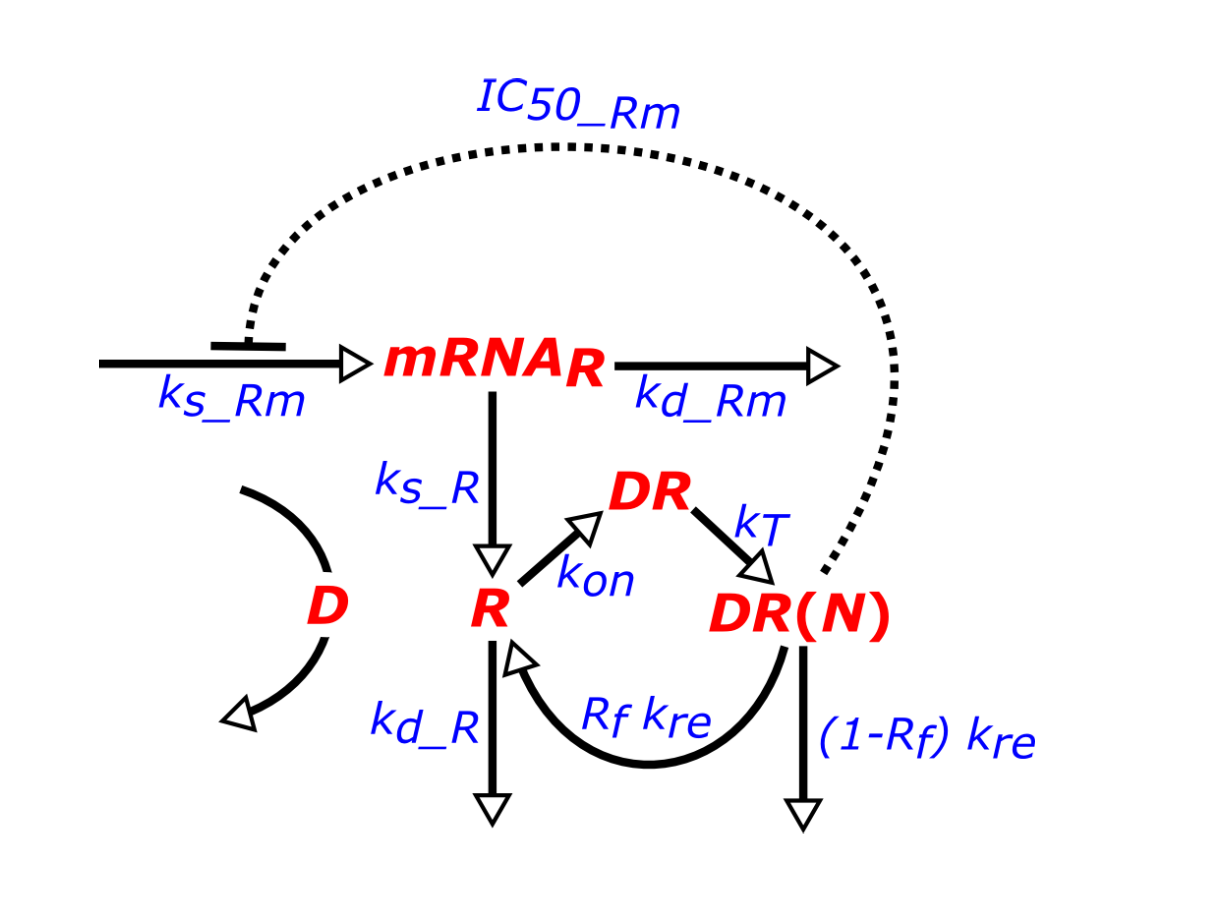
\includegraphics[width=17.11in]{mrna_dynamics} Hierin is duidelijk te
zien dat ksr en kon pas na de mRNAr zich in het biologische proces mengt
omtrent het corticoïde model.

Question 2.4

De code hieronder genereert grafieken die een scenario uitbeelt waarbij
de synthese van de receptor geblokeerd word. De parameter die hiervoor
veranderd moet worden is ks\_r. Dit is omdat deze waarde in de 2e
afgeleide de hoeveelheid receptor regelt. Als we ks\_r dus op 0 zetten
maken we een situatie waarbij er geen synthese meer is van de receptor.

\begin{Shaded}
\begin{Highlighting}[]
\FunctionTok{par}\NormalTok{(}\AttributeTok{mfrow =} \FunctionTok{c}\NormalTok{(}\DecValTok{2}\NormalTok{,}\DecValTok{2}\NormalTok{) )}

\NormalTok{parameters }\OtherTok{\textless{}{-}} \FunctionTok{c}\NormalTok{(}\AttributeTok{ks\_Rm =} \DecValTok{0}\NormalTok{, }\AttributeTok{IC50\_Rm =} \FloatTok{26.2}\NormalTok{, }\AttributeTok{kon =} \FloatTok{0.00329}\NormalTok{,}
                \AttributeTok{kT =} \FloatTok{0.63}\NormalTok{, }\AttributeTok{kre =} \FloatTok{0.57}\NormalTok{, }\AttributeTok{Rf =} \FloatTok{0.49}\NormalTok{, }\AttributeTok{kd\_R =} \FloatTok{0.0572}\NormalTok{,}
                \AttributeTok{kd\_Rm =} \FloatTok{0.612}\NormalTok{, }\AttributeTok{ks\_r =} \DecValTok{0}\NormalTok{, }\AttributeTok{D =} \DecValTok{53}\NormalTok{, }\AttributeTok{Rm0 =} \FloatTok{4.74}\NormalTok{,}
                \AttributeTok{DR =} \DecValTok{0}\NormalTok{, }\AttributeTok{DRN =} \DecValTok{0}\NormalTok{)}

\NormalTok{t }\OtherTok{=} \FunctionTok{seq}\NormalTok{(}\DecValTok{0}\NormalTok{, }\DecValTok{48}\NormalTok{, }\AttributeTok{by =} \FloatTok{0.1}\NormalTok{)}

\NormalTok{out }\OtherTok{\textless{}{-}}\NormalTok{ deSolve}\SpecialCharTok{::}\FunctionTok{ode}\NormalTok{(}\AttributeTok{times =}\NormalTok{ t, }\AttributeTok{y =}\NormalTok{ state, }\AttributeTok{parms =}\NormalTok{ parameters,}
                    \AttributeTok{func =}\NormalTok{ Glucocorticoid\_func, }\AttributeTok{method =} \StringTok{"lsoda"}\NormalTok{)}


\NormalTok{out }\OtherTok{\textless{}{-}} \FunctionTok{as.data.frame}\NormalTok{(out)}

\FunctionTok{plot}\NormalTok{(out}\SpecialCharTok{$}\NormalTok{time,out}\SpecialCharTok{$}\NormalTok{mRNAr,}\AttributeTok{ylim =} \FunctionTok{c}\NormalTok{(}\DecValTok{0}\NormalTok{,}\DecValTok{5}\NormalTok{), }\AttributeTok{xlab=}\StringTok{"Time"}\NormalTok{,}\AttributeTok{ylab=}\StringTok{"receptor mRNA"}\NormalTok{,}\AttributeTok{type=}\StringTok{"l"}\NormalTok{,}\AttributeTok{lwd=}\DecValTok{2}\NormalTok{)}
\FunctionTok{plot}\NormalTok{(out}\SpecialCharTok{$}\NormalTok{time,out}\SpecialCharTok{$}\NormalTok{R, }\AttributeTok{ylim =} \FunctionTok{c}\NormalTok{(}\DecValTok{0}\NormalTok{,}\DecValTok{300}\NormalTok{), }\AttributeTok{xlab=}\StringTok{"Time"}\NormalTok{,}\AttributeTok{ylab=}\StringTok{"free receptor density"}\NormalTok{,}\AttributeTok{type=}\StringTok{"l"}\NormalTok{,}\AttributeTok{lwd=}\DecValTok{2}\NormalTok{)}
\FunctionTok{plot}\NormalTok{(out}\SpecialCharTok{$}\NormalTok{time,out}\SpecialCharTok{$}\NormalTok{DR, }\AttributeTok{ylim =} \FunctionTok{c}\NormalTok{(}\DecValTok{0}\NormalTok{,}\DecValTok{50}\NormalTok{), }\AttributeTok{xlab=}\StringTok{"Time"}\NormalTok{,}\AttributeTok{ylab=}\StringTok{"drug{-}receptor complex"}\NormalTok{,}\AttributeTok{type=}\StringTok{"l"}\NormalTok{,}\AttributeTok{lwd=}\DecValTok{2}\NormalTok{)}
\FunctionTok{plot}\NormalTok{(out}\SpecialCharTok{$}\NormalTok{time,out}\SpecialCharTok{$}\NormalTok{DRN, }\AttributeTok{ylim =} \FunctionTok{c}\NormalTok{(}\DecValTok{0}\NormalTok{,}\DecValTok{50}\NormalTok{), }\AttributeTok{xlab=}\StringTok{"Time"}\NormalTok{,}\AttributeTok{ylab=}\StringTok{"activated receptor complex"}\NormalTok{,}\AttributeTok{type=}\StringTok{"l"}\NormalTok{,}\AttributeTok{lwd=}\DecValTok{2}\NormalTok{)}
\end{Highlighting}
\end{Shaded}

\includegraphics{Project-Thema08-week3-Groep2_v1_files/figure-latex/unnamed-chunk-7-1.pdf}
Voornamelijk in de figuren onderaan is te zien dat de drug- en activated
receptor dichtheid vrij snel daalt omdat de synthese van de receptor
geblokeerd is. Als je dit vergelijkt met de normale situatie is er zeker
een verschil.

Question 2.5

In dit scenario kijken we naar wat er gebeurt als we de parameters,
ks\_rm en kd\_rm vergroten en verkleinen. We testen dit met de volgende
`fold changes': / 2, / 5, x 2 en x 5. Hier onder is de code te zien die
deze situatie tot leven brengt:

\begin{Shaded}
\begin{Highlighting}[]
\FunctionTok{par}\NormalTok{(}\AttributeTok{mfrow =} \FunctionTok{c}\NormalTok{(}\DecValTok{2}\NormalTok{,}\DecValTok{2}\NormalTok{) )}
\NormalTok{t }\OtherTok{\textless{}{-}} \FunctionTok{seq}\NormalTok{(}\DecValTok{0}\NormalTok{, }\DecValTok{50}\NormalTok{, }\AttributeTok{by =} \FloatTok{0.1}\NormalTok{)}

\NormalTok{parameters\_1 }\OtherTok{\textless{}{-}} \FunctionTok{c}\NormalTok{(}\AttributeTok{ks\_Rm =} \FloatTok{2.90}\SpecialCharTok{/}\DecValTok{5}\NormalTok{, }\AttributeTok{IC50\_Rm =} \FloatTok{26.2}\NormalTok{, }\AttributeTok{kon =} \FloatTok{0.00329}\NormalTok{,}
                \AttributeTok{kT =} \FloatTok{0.63}\NormalTok{, }\AttributeTok{kre =} \FloatTok{0.57}\NormalTok{, }\AttributeTok{Rf =} \FloatTok{0.49}\NormalTok{, }\AttributeTok{kd\_R =} \FloatTok{0.0572}\NormalTok{,}
                \AttributeTok{kd\_Rm =} \FloatTok{2.9}\SpecialCharTok{/}\DecValTok{5}\SpecialCharTok{/}\FloatTok{4.74}\NormalTok{, }\AttributeTok{ks\_r =} \FloatTok{3.22}\NormalTok{, }\AttributeTok{D =} \DecValTok{53}\NormalTok{, }\AttributeTok{Rm0 =} \FloatTok{4.74}\NormalTok{,}
                \AttributeTok{DR =} \DecValTok{0}\NormalTok{, }\AttributeTok{DRN =} \DecValTok{0}\NormalTok{)}

\NormalTok{parameters\_2 }\OtherTok{\textless{}{-}} \FunctionTok{c}\NormalTok{(}\AttributeTok{ks\_Rm =} \FloatTok{2.90}\SpecialCharTok{/}\DecValTok{2}\NormalTok{, }\AttributeTok{IC50\_Rm =} \FloatTok{26.2}\NormalTok{, }\AttributeTok{kon =} \FloatTok{0.00329}\NormalTok{,}
                \AttributeTok{kT =} \FloatTok{0.63}\NormalTok{, }\AttributeTok{kre =} \FloatTok{0.57}\NormalTok{, }\AttributeTok{Rf =} \FloatTok{0.49}\NormalTok{, }\AttributeTok{kd\_R =} \FloatTok{0.0572}\NormalTok{,}
                \AttributeTok{kd\_Rm =} \FloatTok{2.9}\SpecialCharTok{/}\DecValTok{2}\SpecialCharTok{/}\FloatTok{4.74}\NormalTok{, }\AttributeTok{ks\_r =} \FloatTok{3.22}\NormalTok{, }\AttributeTok{D =} \DecValTok{53}\NormalTok{, }\AttributeTok{Rm0 =} \FloatTok{4.74}\NormalTok{,}
                \AttributeTok{DR =} \DecValTok{0}\NormalTok{, }\AttributeTok{DRN =} \DecValTok{0}\NormalTok{)}

\NormalTok{parameters\_3 }\OtherTok{\textless{}{-}} \FunctionTok{c}\NormalTok{(}\AttributeTok{ks\_Rm =} \FloatTok{2.90}\SpecialCharTok{*}\DecValTok{2}\NormalTok{, }\AttributeTok{IC50\_Rm =} \FloatTok{26.2}\NormalTok{, }\AttributeTok{kon =} \FloatTok{0.00329}\NormalTok{,}
                \AttributeTok{kT =} \FloatTok{0.63}\NormalTok{, }\AttributeTok{kre =} \FloatTok{0.57}\NormalTok{, }\AttributeTok{Rf =} \FloatTok{0.49}\NormalTok{, }\AttributeTok{kd\_R =} \FloatTok{0.0572}\NormalTok{,}
                \AttributeTok{kd\_Rm =} \FloatTok{2.9}\SpecialCharTok{*}\DecValTok{2}\SpecialCharTok{/}\FloatTok{4.74}\NormalTok{, }\AttributeTok{ks\_r =} \FloatTok{3.22}\NormalTok{, }\AttributeTok{D =} \DecValTok{53}\NormalTok{, }\AttributeTok{Rm0 =} \FloatTok{4.74}\NormalTok{,}
                \AttributeTok{DR =} \DecValTok{0}\NormalTok{, }\AttributeTok{DRN =} \DecValTok{0}\NormalTok{)}

\NormalTok{parameters\_4 }\OtherTok{\textless{}{-}} \FunctionTok{c}\NormalTok{(}\AttributeTok{ks\_Rm =} \FloatTok{2.90}\SpecialCharTok{*}\DecValTok{5}\NormalTok{, }\AttributeTok{IC50\_Rm =} \FloatTok{26.2}\NormalTok{, }\AttributeTok{kon =} \FloatTok{0.00329}\NormalTok{,}
                \AttributeTok{kT =} \FloatTok{0.63}\NormalTok{, }\AttributeTok{kre =} \FloatTok{0.57}\NormalTok{, }\AttributeTok{Rf =} \FloatTok{0.49}\NormalTok{, }\AttributeTok{kd\_R =} \FloatTok{0.0572}\NormalTok{,}
                \AttributeTok{kd\_Rm =} \FloatTok{2.9}\SpecialCharTok{*}\DecValTok{5}\SpecialCharTok{/}\FloatTok{4.74}\NormalTok{, }\AttributeTok{ks\_r =} \FloatTok{3.22}\NormalTok{, }\AttributeTok{D =} \DecValTok{53}\NormalTok{, }\AttributeTok{Rm0 =} \FloatTok{4.74}\NormalTok{,}
                \AttributeTok{DR =} \DecValTok{0}\NormalTok{, }\AttributeTok{DRN =} \DecValTok{0}\NormalTok{)}

\NormalTok{out\_1 }\OtherTok{\textless{}{-}}\NormalTok{ deSolve}\SpecialCharTok{::}\FunctionTok{ode}\NormalTok{(}\AttributeTok{times =}\NormalTok{ t, }\AttributeTok{y =}\NormalTok{ state, }\AttributeTok{parms =}\NormalTok{ parameters\_1,}
                    \AttributeTok{func =}\NormalTok{ Glucocorticoid\_func, }\AttributeTok{method =} \StringTok{"lsoda"}\NormalTok{)}

\NormalTok{out\_2 }\OtherTok{\textless{}{-}}\NormalTok{ deSolve}\SpecialCharTok{::}\FunctionTok{ode}\NormalTok{(}\AttributeTok{times =}\NormalTok{ t, }\AttributeTok{y =}\NormalTok{ state, }\AttributeTok{parms =}\NormalTok{ parameters\_2,}
                    \AttributeTok{func =}\NormalTok{ Glucocorticoid\_func, }\AttributeTok{method =} \StringTok{"lsoda"}\NormalTok{)}

\NormalTok{out\_3 }\OtherTok{\textless{}{-}}\NormalTok{ deSolve}\SpecialCharTok{::}\FunctionTok{ode}\NormalTok{(}\AttributeTok{times =}\NormalTok{ t, }\AttributeTok{y =}\NormalTok{ state, }\AttributeTok{parms =}\NormalTok{ parameters\_3,}
                    \AttributeTok{func =}\NormalTok{ Glucocorticoid\_func, }\AttributeTok{method =} \StringTok{"lsoda"}\NormalTok{)}

\NormalTok{out\_4 }\OtherTok{\textless{}{-}}\NormalTok{ deSolve}\SpecialCharTok{::}\FunctionTok{ode}\NormalTok{(}\AttributeTok{times =}\NormalTok{ t, }\AttributeTok{y =}\NormalTok{ state, }\AttributeTok{parms =}\NormalTok{ parameters\_4,}
                    \AttributeTok{func =}\NormalTok{ Glucocorticoid\_func, }\AttributeTok{method =} \StringTok{"lsoda"}\NormalTok{)}

\NormalTok{out\_1 }\OtherTok{\textless{}{-}} \FunctionTok{as.data.frame}\NormalTok{(out\_1)}
\NormalTok{out\_2 }\OtherTok{\textless{}{-}} \FunctionTok{as.data.frame}\NormalTok{(out\_2)}
\NormalTok{out\_3 }\OtherTok{\textless{}{-}} \FunctionTok{as.data.frame}\NormalTok{(out\_3)}
\NormalTok{out\_4 }\OtherTok{\textless{}{-}} \FunctionTok{as.data.frame}\NormalTok{(out\_4)}

\FunctionTok{plot}\NormalTok{(out\_1}\SpecialCharTok{$}\NormalTok{time, out\_1}\SpecialCharTok{$}\NormalTok{mRNAr,}
     \AttributeTok{ylab=}\FunctionTok{c}\NormalTok{(}\StringTok{"Receptor mRNA"}\NormalTok{), }\AttributeTok{xlab=}\FunctionTok{c}\NormalTok{(}\StringTok{" Time in hours"}\NormalTok{),}
     \AttributeTok{type=}\StringTok{\textquotesingle{}l\textquotesingle{}}\NormalTok{, }\AttributeTok{lwd =} \DecValTok{2}\NormalTok{, }\AttributeTok{xlim=} \FunctionTok{c}\NormalTok{(}\DecValTok{0}\NormalTok{,}\DecValTok{50}\NormalTok{), }\AttributeTok{ylim=} \FunctionTok{c}\NormalTok{(}\DecValTok{5}\NormalTok{, }\DecValTok{0}\NormalTok{))}

\FunctionTok{lines}\NormalTok{(out\_2}\SpecialCharTok{$}\NormalTok{time, out\_2}\SpecialCharTok{$}\NormalTok{mRNAr, }\AttributeTok{lwd =} \DecValTok{2}\NormalTok{, }\AttributeTok{col =} \StringTok{"red"}\NormalTok{)}
\FunctionTok{lines}\NormalTok{(out\_3}\SpecialCharTok{$}\NormalTok{time, out\_3}\SpecialCharTok{$}\NormalTok{mRNAr, }\AttributeTok{lwd =} \DecValTok{2}\NormalTok{, }\AttributeTok{col =} \StringTok{"blue"}\NormalTok{)}
\FunctionTok{lines}\NormalTok{(out\_4}\SpecialCharTok{$}\NormalTok{time, out\_4}\SpecialCharTok{$}\NormalTok{mRNAr, }\AttributeTok{lwd =} \DecValTok{2}\NormalTok{, }\AttributeTok{col =} \StringTok{"purple"}\NormalTok{)}

\FunctionTok{plot}\NormalTok{(out\_1}\SpecialCharTok{$}\NormalTok{time, out\_1}\SpecialCharTok{$}\NormalTok{R,}
     \AttributeTok{ylab=}\FunctionTok{c}\NormalTok{(}\StringTok{"Free receptor density"}\NormalTok{), }\AttributeTok{xlab=}\FunctionTok{c}\NormalTok{(}\StringTok{" Time in hours"}\NormalTok{),}
     \AttributeTok{type=}\StringTok{\textquotesingle{}l\textquotesingle{}}\NormalTok{, }\AttributeTok{lwd =} \DecValTok{2}\NormalTok{, }\AttributeTok{xlim=} \FunctionTok{c}\NormalTok{(}\DecValTok{0}\NormalTok{,}\DecValTok{50}\NormalTok{), }\AttributeTok{ylim=} \FunctionTok{c}\NormalTok{(}\DecValTok{0}\NormalTok{, }\DecValTok{400}\NormalTok{))}

\FunctionTok{lines}\NormalTok{(out\_2}\SpecialCharTok{$}\NormalTok{time, out\_2}\SpecialCharTok{$}\NormalTok{R, }\AttributeTok{lwd =} \DecValTok{2}\NormalTok{, }\AttributeTok{col =} \StringTok{"red"}\NormalTok{)}
\FunctionTok{lines}\NormalTok{(out\_3}\SpecialCharTok{$}\NormalTok{time, out\_3}\SpecialCharTok{$}\NormalTok{R, }\AttributeTok{lwd =} \DecValTok{2}\NormalTok{, }\AttributeTok{col =} \StringTok{"blue"}\NormalTok{)}
\FunctionTok{lines}\NormalTok{(out\_4}\SpecialCharTok{$}\NormalTok{time, out\_4}\SpecialCharTok{$}\NormalTok{R, }\AttributeTok{lwd =} \DecValTok{2}\NormalTok{, }\AttributeTok{col =} \StringTok{"purple"}\NormalTok{)}

\FunctionTok{plot}\NormalTok{(out\_1}\SpecialCharTok{$}\NormalTok{time, out\_1}\SpecialCharTok{$}\NormalTok{DR,}
     \AttributeTok{ylab=}\FunctionTok{c}\NormalTok{(}\StringTok{"Drug{-}receoptor complex"}\NormalTok{), }\AttributeTok{xlab=}\FunctionTok{c}\NormalTok{(}\StringTok{" Time in hours"}\NormalTok{),}
     \AttributeTok{type=}\StringTok{\textquotesingle{}l\textquotesingle{}}\NormalTok{, }\AttributeTok{lwd =} \DecValTok{2}\NormalTok{, }\AttributeTok{xlim=} \FunctionTok{c}\NormalTok{(}\DecValTok{0}\NormalTok{,}\DecValTok{50}\NormalTok{), }\AttributeTok{ylim=} \FunctionTok{c}\NormalTok{(}\DecValTok{50}\NormalTok{, }\SpecialCharTok{{-}}\DecValTok{50}\NormalTok{))}

\FunctionTok{lines}\NormalTok{(out\_2}\SpecialCharTok{$}\NormalTok{time, out\_2}\SpecialCharTok{$}\NormalTok{DR, }\AttributeTok{lwd =} \DecValTok{2}\NormalTok{, }\AttributeTok{col =} \StringTok{"red"}\NormalTok{)}
\FunctionTok{lines}\NormalTok{(out\_3}\SpecialCharTok{$}\NormalTok{time, out\_3}\SpecialCharTok{$}\NormalTok{DR, }\AttributeTok{lwd =} \DecValTok{2}\NormalTok{, }\AttributeTok{col =} \StringTok{"blue"}\NormalTok{)}
\FunctionTok{lines}\NormalTok{(out\_4}\SpecialCharTok{$}\NormalTok{time, out\_4}\SpecialCharTok{$}\NormalTok{DR, }\AttributeTok{lwd =} \DecValTok{2}\NormalTok{, }\AttributeTok{col =} \StringTok{"purple"}\NormalTok{)}

\FunctionTok{plot}\NormalTok{(out\_1}\SpecialCharTok{$}\NormalTok{time, out\_1}\SpecialCharTok{$}\NormalTok{DRN,}
     \AttributeTok{ylab=}\FunctionTok{c}\NormalTok{(}\StringTok{"Activated receptor complex"}\NormalTok{), }\AttributeTok{xlab=}\FunctionTok{c}\NormalTok{(}\StringTok{" Time in hours"}\NormalTok{),}
     \AttributeTok{type=}\StringTok{\textquotesingle{}l\textquotesingle{}}\NormalTok{, }\AttributeTok{lwd =} \DecValTok{2}\NormalTok{, }\AttributeTok{xlim=} \FunctionTok{c}\NormalTok{(}\DecValTok{0}\NormalTok{,}\DecValTok{50}\NormalTok{), }\AttributeTok{ylim=} \FunctionTok{c}\NormalTok{(}\DecValTok{50}\NormalTok{, }\SpecialCharTok{{-}}\DecValTok{50}\NormalTok{))}

\FunctionTok{lines}\NormalTok{(out\_2}\SpecialCharTok{$}\NormalTok{time, out\_2}\SpecialCharTok{$}\NormalTok{DRN, }\AttributeTok{lwd =} \DecValTok{2}\NormalTok{, }\AttributeTok{col =} \StringTok{"red"}\NormalTok{)}
\FunctionTok{lines}\NormalTok{(out\_3}\SpecialCharTok{$}\NormalTok{time, out\_3}\SpecialCharTok{$}\NormalTok{DRN, }\AttributeTok{lwd =} \DecValTok{2}\NormalTok{, }\AttributeTok{col =} \StringTok{"blue"}\NormalTok{)}
\FunctionTok{lines}\NormalTok{(out\_4}\SpecialCharTok{$}\NormalTok{time, out\_4}\SpecialCharTok{$}\NormalTok{DRN, }\AttributeTok{lwd =} \DecValTok{2}\NormalTok{, }\AttributeTok{col =} \StringTok{"purple"}\NormalTok{)}
\end{Highlighting}
\end{Shaded}

\includegraphics{Project-Thema08-week3-Groep2_v1_files/figure-latex/unnamed-chunk-8-1.pdf}
In de plotjes hierboven is vooral bij de figuur linksboven een duidelijk
verschil te zien tussen de fold changes. Dus de receptor mRNA hangt het
meest af van de ks\_rm \& kd\_rm parameters af in vergelijking met de
andere figuren. De kleuren duiden de hoeveelheid change aan: zwart = x
5, rood = x 2, blauw = / 2 en paars is / 5.

\hypertarget{discussion-and-conclusion}{%
\section{Discussion and Conclusion}\label{discussion-and-conclusion}}

\hypertarget{discussion}{%
\subsection{Discussion}\label{discussion}}

\begin{itemize}
\tightlist
\item
  Compare your results with what is expecting from the literature and
  discuss differences with them.
\end{itemize}

Vergeleken met de literaire resultaten zijn er veel overeenkomsten.
Enige verschillen zijn de gegevens (cijfers) uit dit verslag t.o.v. de
steekproefgegevens uit de voorbeelden. Waardoor de prognoses (modellen
en grafieken) verschillen met de originele cijfers

Om het model preciezer te maken zou er meer achtergrond informatie
moeten worden opgedaan en geïmplementeerd, aangezien de theorie nu uit
slechts vier bronnen plus een aangereikte bron van de vakdocent
betreffen.

Al met al is, middels het testen, en door verschillende parameters te
gebruiken plus verschillende geproduceerde resultaten, het model wel
significant betrouwbaar en praktisch toepasbaar voor nader onderzoek.

\hypertarget{general-conclusion-and-perspective}{%
\subsection{General conclusion and
perspective}\label{general-conclusion-and-perspective}}

Het doel van deze opdracht was uitbouwen op de eigen-implementatie van
het corticoide model, door additionele simulaties uit te voeren. Om deze
tot slot in detail te vergelijken met andere resultaten. Vanuit deze
progressie is het belangrijk om de onderzoeksresultaten te valideren,
dat zal gebeuren in de volgende opdracht. Waar we `peer reviiews' zullen
houden.

\end{document}
